%CHAPTER 6
\chapterfigure[width=\linewidth]{Durer/Durer_Revelation_Four_Riders.jpg}[Los Cuatro Jinetes]{Los Cuatro Jinetes. Albrecht Dürer, 1498.}

\chapter{Los Primeros Seis Sellos}
\subsubsection*{El Primer Sello}
\lettrine[lines=3,slope=-0.5em,loversize=0.1]{\textcolor{red}{Y}}{\hspace{0.5em} miré} cuando el Cordero abrió uno de los sellos, y oí a uno los cuatro animales diciendo como con una voz de trueno: Ven y ve. 
\vnum{2}Y miré, y he aquí un caballo blanco:%
	\cbiblefootduosb{Zechariah}{1:8-11}{Vi de noche, y he aquí un varón que cabalgaba sobre un caballo bermejo, el cual estaba entre los mirtos\ldots y detrás de él había caballos bermejos, overos, y blancos\ldots Y aquel varón que estaba entre los mirtos\ldots dijo: Estos son los que Jehová ha enviado a recorrer la tierra. Y ellos hablaron a aquel ángel de Jehová que estaba entre los mirtos, y dijeron: Hemos recorrido la tierra, y he aquí toda la tierra está reposada y quieta}%
					{6:1-8}{He aquí cuatro carros que salían de entre dos montes\ldots En el primer carro había caballos bermejos, y el segundo carro caballos negros, y en el tercer carro caballos blancos, y en el cuarto carro caballos overos ruciorodados\ldots Estos son los cuatro vientos de los cielos, que salen de donde están delante del Señor de toda la tierra\ldots y dijo: Id, recorred la tierra. Y recorrieron la tierra}
 y el que estaba sentado encima de él, tenía un arco; y le fue dada una corona, y salió victorioso, para que también venciese.
\subsubsection*{El Segundo Sello}
\vnum{3}Y cuando él abrió el segundo sello, oí al segundo animal, que decía: Ven y ve. %
\vnum{4}Y salió otro caballo bermejo: y al que estaba sentado sobre él, fue dado poder de quitar la paz de la tierra, y que se maten unos a otros: y fuele dada una grande espada.
\subsubsection*{El Tercer Sello}
\vnum{5}Y cuando él abrió el tercer sello, oí al tercer animal, que decía: Ven y ve. Y miré, y he aquí un caballo negro: y el que estaba sentado encima de él, tenía un peso en su mano. %
\vnum{6}Y oí una voz en medio de los cuatro animales, que decía: Dos libras de trigo por un denario, y seis libras de cebada por un denario: y no hagas daño al vino ni al aceite.
\subsubsection*{El Cuarto Sello}
\vnum{7}Y cuando él abrió el cuarto sello, oí la voz del cuarto animal, que decía: Ven y ve. %
\vnum{8}Y miré, y he aquí un caballo amarillo: y el que estaba sentado sobre él tenía por nombre Muerte; y el infierno le seguía: y le fue dada potestad sobre la cuarta parte de la tierra, para matar con espada, con hambre, con mortandad, y con las bestias de la tierra.%
	\footnote{\cbibleref{Ezekiel}{5:12, 17}{Una tercera parte de ti morirá de pestilencia, y de hambre será consumida en medio de ti; y una tercera parte caerá a cuchillo alrededor de ti; y una tercera parte esparciré a todos los vientos, y tras ellos desenvainaré espada\ldots Enviaré pues sobre vosotros hambre, y malas bestias que te destruyan; y pestilencia y sangre pasarán por ti; y meteré sobre ti cuchillo. Yo Jehová he hablado} %
			\cbiblechvs{Ezekiel}{14:21}{¿Cuánto más, si mis cuatro malos juicios, espada, y hambre, y mala bestia, y pestilencia, enviare contra Jerusalem, para talar de ella hombres y bestias?} %
			\cbiblechvs{Ezekiel}{33:27}{Así ha dicho el Señor Jehová: Vivo yo, que los que están en aquellos asolamientos caerán a cuchillo, y al que está sobre la haz del campo entregaré a las bestias que lo devoren; y los que están en las fortalezas y en las cuevas, de pestilencia morirán} %
			\cbibleref{Jeremiah}{14:12}{Los consumiré con cuchillo, y con hambre, y con pestilencia} %
			\cbiblechvs{Jeremiah}{15:2-3}{Así ha dicho Jehová: El que a muerte, a muerte; y el que a cuchillo, a cuchillo; y el que a hambre, a hambre; y el que a cautividad, a cautividad. Y enviaré sobre ellos cuatro géneros, dice Jehová: cuchillo para matar, y perros para despedazar, y aves del cielo y bestias de la tierra, para devorar y para disipar}
			}%
\subsubsection*{El Quinto Sello}
\vnum{9}Y cuando él abrió el quinto sello, vi debajo del altar las almas de los que habían sido muertos por la palabra de Dios y por el testimonio que ellos tenían. %
\vnum{10}Y clamaban en alta voz diciendo: ¿Hasta cuándo, Señor, santo y verdadero,%
	\cbiblefootduo{Psalms}{79:1-6}{Oh Dios, vinieron las gentes a tu heredad; el templo de tu santidad han contaminado; pusieron a Jerusalem en montones. Dieron los cuerpos de tus siervos por comida a las aves de los cielos; la carne de tus santos a las bestias de la tierra. Derramaron su sangre como agua en los alrededores de Jerusalem; y no hubo quien los enterrase. Somos afrentados de nuestros vecinos, escarnecidos y burlados de los que están en nuestros alrededores. ¿Hasta cuándo, oh Jehová? ¿has de estar airado para siempre? ¿Arderá como fuego tu celo? Derrama tu ira sobre las gentes que no te conocen, y sobre los reinos que no invocan tu nombre}%
				{Zechariah}{1:12}{El ángel de Jehová\ldots dijo: Oh Jehová de los ejércitos, ¿hasta cuándo no tendrás piedad de Jerusalem, y de las ciudades de Judá, con las cuales has estado airado por espacio de setenta años?}
 no juzgas y vengas nuestra sangre de los que moran en la tierra?%
 	\footnote{\cbibleref{Psalms}{79:10-13}{Porque dirán las gentes: ¿Dónde está su Dios? Sea notoria en las gentes, delante de nuestros ojos, la venganza de la sangre de tus siervos, que fue derramada. Entre ante tu acatamiento el gemido de los presos: conforme a la grandeza de tu brazo preserva a los sentenciados a muerte. Y torna a nuestros vecinos en su seno siete tantos de su infamia, con que te han deshonrado, oh Jehová. Y nosotros, pueblo tuyo, y ovejas de tu dehesa, te alabaremos para siempre: por generación y generación cantaremos tus alabanzas}
 	} %
\vnum{11}Y les fueron dadas sendas ropas blancas, y fuéles dicho que reposasen todavía un poco de tiempo, hasta que se completaran sus consiervos y sus hermanos, que también habían de ser muertos como ellos.
\subsubsection*{El Sexto Sello}
\vnum{12}Y miré cuando él abrió el sexto sello, y he aquí fue hecho un gran terremoto;%
	\cbiblefoot{Ezekiel}{38:19-20}{He hablado en mi celo, y en el fuego de mi ira: Que en aquel tiempo habrá gran temblor sobre la tierra de Israel; que los peces de la mar, y las aves del cielo, y las bestias del campo, y toda serpiente que anda arrastrando sobre la tierra, y todos los hombres que están sobre la haz de la tierra, temblarán a mi presencia; y se arruinarán los montes, y los vallados caerán, y todo muro caerá a tierra}
 y el sol se puso negro como un saco de cilicio, y la luna se puso toda como sangre;%
 	\footnote{
 		\cbibleref{Joel}{3:14-16}{Cercano está el día de Jehová en el valle de la decisión. El sol y la luna se oscurecerán, y las estrellas retraerán su resplandor. Y Jehová bramará desde Sión, y dará su voz desde Jerusalem} %
 		\cbibleref{Isaiah}{13:9-11, 13}{He aquí el día de Jehová viene, crudo, y de saña y ardor de ira, para tornar la tierra en soledad, y raer de ella sus pecadores. Por lo cual las estrellas de los cielos y sus luceros no derramarán su lumbre; y el sol se oscurecerá en naciendo, y la luna no echará su resplandor. Y visitaré la maldad sobre el mundo, y sobre los impíos su iniquidad; y haré que cese la arrogancia de los soberbios, y abatiré la altivez de los fuertes\ldots Porque haré estremecer los cielos, y la tierra se moverá de su lugar, en la indignación de Jehová de los ejércitos, y en el día de la ira de su furor} %
 		\cbiblechvs{Isaiah}{50:2-3}{He aquí que con mi reprensión\ldots visto de oscuridad los cielos, y torno como saco su cobertura} % 		
 		\cbibleref{Ezekiel}{32:7-9}{Cuando te habré muerto, cubriré los cielos, y haré entenebrecer sus estrellas: el sol cubriré con nublado, y la luna no hará resplandecer su luz. Todas las lumbreras de luz haré entenebrecer en el cielo por ti, y pondré tinieblas sobre tu tierra, dice el Señor Jehová. Y entristeceré el corazón de muchos pueblos, cuando llevaré tu quebrantamiento sobre las gentes, por las tierras que no conociste}%
 	} %
\vnum{13}y las estrellas del cielo cayeron sobre la tierra, como la higuera echa sus higos cuando es movida de gran viento.%
	\cbiblefoot{Isaiah}{34:2-6}{Jehová está airado sobre todas las gentes, é irritado sobre todo el ejército de ellas: destruirálas y entregarálas al matadero por la sangre de ellos. Y los muertos de ellas serán arrojados, y de sus cadáveres se levantará hedor; y los montes se desleirán por la sangre de ellos. Y todo el ejército de los cielos se corromperá, y plegarse han los cielos como un libro: y caerá todo su ejército, como se cae la hoja de la parra, y como se cae la de la higuera. Porque en los cielos se embriagará mi espada: he aquí que descenderá\ldots sobre el pueblo de mi anatema} %
\vnum{14}Y el cielo se apartó como un libro que es envuelto; y todo monte y las islas fueron movidas de sus lugares.%
	\cbiblefoot{Ezekiel}{26:15}{Así ha dicho el Señor Jehová a Tiro: ¿No se estremecerán las islas al estruendo de tu caída, cuando gritarán los heridos, cuando se hará la matanza en medio de ti?} %
\vnum{15}Y los reyes de la tierra, y los príncipes, y los ricos, y los capitanes, y los fuertes,%
	\cbiblefootduosb{Isaiah}{24:21}{Acontecerá en aquel día, que Jehová visitará sobre el ejército sublime en lo alto, y sobre los reyes de la tierra que hay sobre la tierra}%
					{34:12}{Llamarán a sus príncipes, príncipes sin reino: y todos sus grandes serán nada}
 y todo siervo y todo libre, se escondieron en las cuevas y entre las peñas de los montes;%
 	\footnote{\cbibleref{Isaiah}{2:9-12}{Hase inclinado el hombre, y el varón se ha humillado: por tanto no los perdonarás. Métete en la piedra, escóndete en el polvo, de la presencia espantosa de Jehová y del resplandor de su majestad. La altivez de los ojos del hombre será abatida, y la soberbia de los hombres será humillada; y Jehová solo será ensalzado en aquel día. Porque día de Jehová de los ejércitos vendrá sobre todo soberbio y altivo, y sobre todo ensalzado; y será abatido} %
 			\cbiblevs{Isaiah}{2:19-21}{Y meteránse en las cavernas de las peñas, y en las aberturas de la tierra, por la presencia espantosa de Jehová, y por el resplandor de su majestad, cuando se levantare él para herir la tierra. Aquel día arrojará el hombre, a los topos y murciélagos, sus ídolos de plata y sus ídolos de oro, que le hicieron para que adorase; y se entrarán en las hendiduras de las rocas y en las cavernas de las peñas, por la presencia formidable de Jehová, y por el resplandor de su majestad, cuando se levantare para herir la tierra}		
 	}
\vnum{16}Y decían a los montes y a las peñas: Caed sobre nosotros, y escondednos de la cara de aquél que está sentado sobre el trono, y de la ira del Cordero: %
\vnum{17}porque el gran día de su ira es venido; ¿y quién podrá estar firme?%
	\footnote{
		\cbibleref{Joel}{2:11}{Grande es el día de Jehová, y muy terrible; ¿y quién lo podrá sufrir?} %
		\cbiblechvs{Joel}{3:14}{Cercano está el día de Jehová en el valle de la decisión} %
		\cbibleref{Zephaniah}{1:14-15}{Cercano está el día grande de Jehová, cercano y muy presuroso; voz amarga del Día de Jehová; gritará allí el valiente. Día de ira aquel día, día de angustia y de aprieto, día de alboroto y de asolamiento} %
		\cbibleref{Nahum}{1:6}{¿Quién permanecerá delante de su ira? ¿y quién quedará en pié en el furor de su enojo? Su ira se derrama como fuego, y por él se hienden las peñas} %
		\cbibleref{Malachi}{3:2}{¿Y quién podrá sufrir el tiempo de su venida? ó ¿quién podrá estar cuando él se mostrará? Porque él es como fuego purificador, y como jabón de lavadores}%
	}

  \begin{figure*}[p]
  	\centering
  	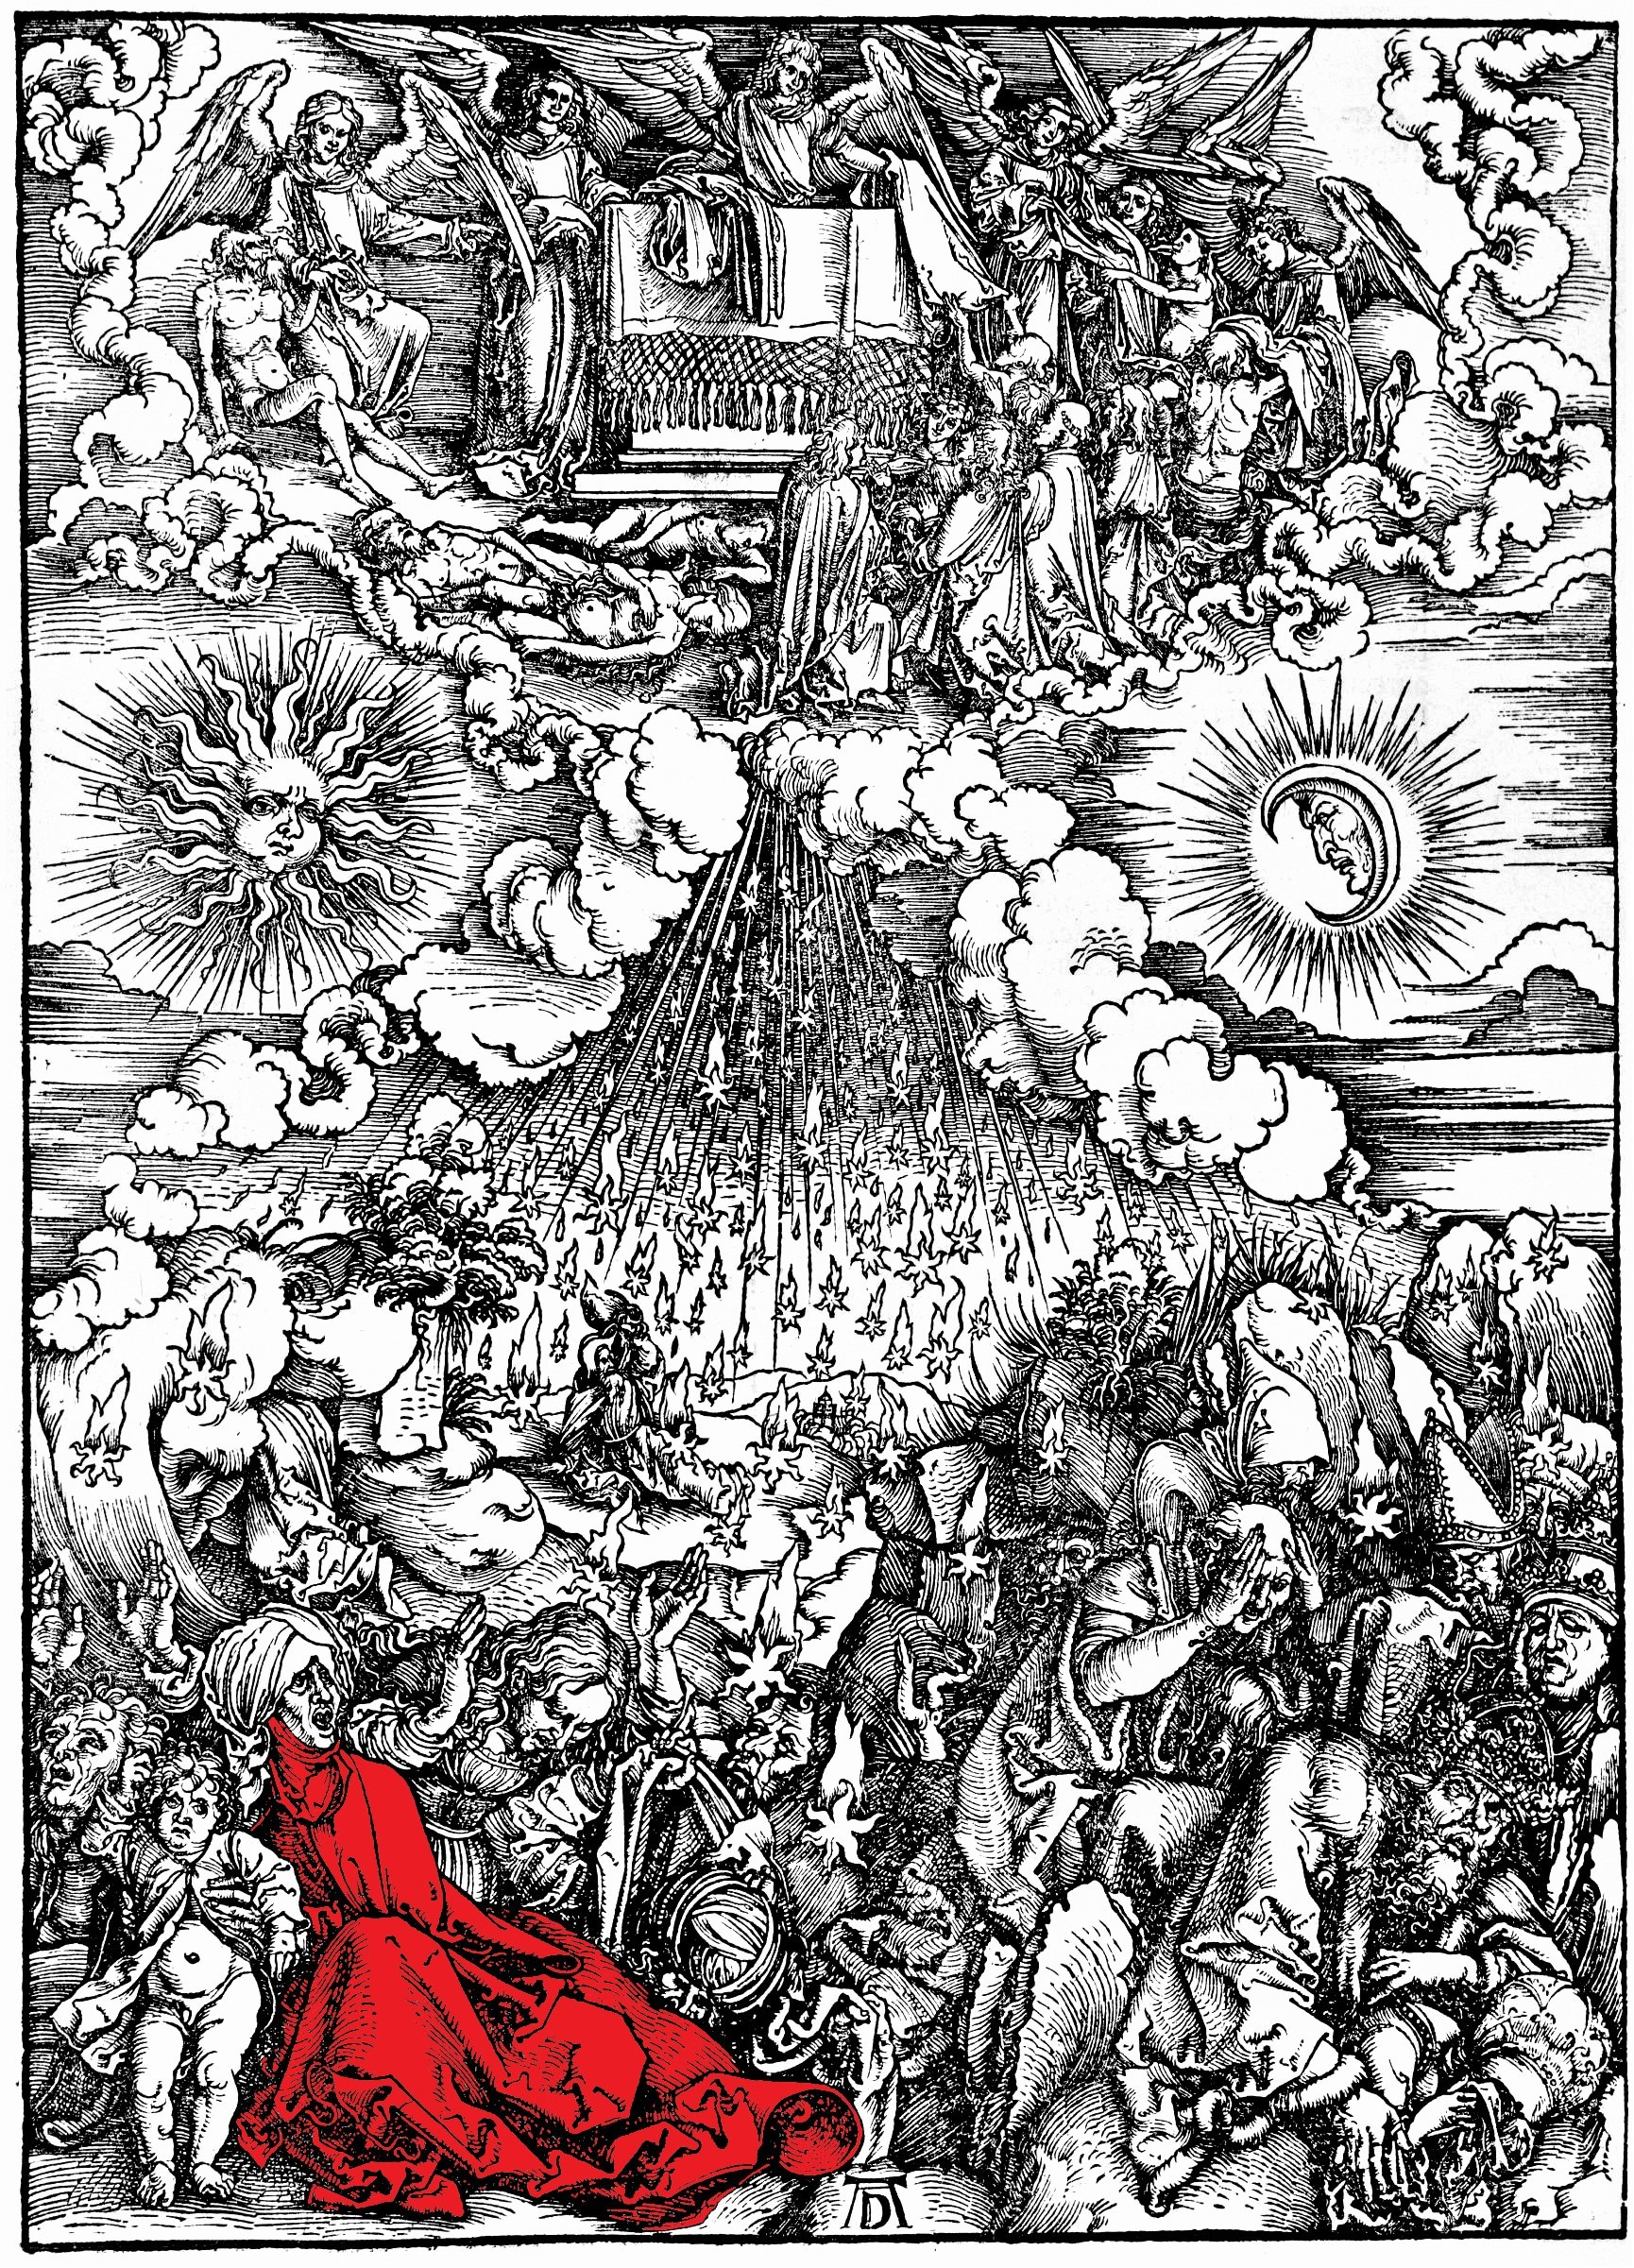
\includegraphics[width=\linewidth]{Durer/Durer_Sixth_Seal.jpg}
  	\caption[La Apertura del Quinto y Sexto Sellos]{La Apertura del Quinto y Sexto Sellos. Albrecht Dürer, 1498.}
  \end{figure*}
